% Kapitel ch:mr: Lead, Setup, Results & Discussion. Setting steht in docs/introduction_v2.tex,
% Discussion in docs/discussion_omol25.md (Conclusion & Outlook).
% Einzige Quelle fuer den Kapiteltext; section_results.tex und
% section_results_merged.tex sind abgeloest.
%
% Gruppennamen: closed-shell (<S^2> = 0) und broken-symmetry (<S^2> > 0),
% klassifiziert nach der Einzelpunktrechnung mit Stabilitaetsanalyse.
% "RKS instability" nur dort, wo der Stabilitaetstest beschrieben ist.
% "restricted surface" / "ground-state surface" sind Flaechen, keine Gruppen.
%
% Figuren: Pictures/Fig1.png, Pictures/fig2_force_mae.png, Pictures/fig3.png
% aus pipeline/plot_paper_figs_v2.py. Zahlen aus results/*.csv, geprueft mit
% pipeline/check_results_section.py.

\chapter{Higher-Fidelity Relabelling Without Re-optimising the Path Is Not Enough}
\label{ch:mr}

The introduction asked two questions: whether a model can be lifted
to a higher level of theory by relabelling only a subset of its
training data (RQ1), and whether a model can learn a surface from
paths that were never relaxed on that surface (RQ2).
Chapter~\ref{ch:delta} answered RQ1. For that chapter, RQ2 needed no
test: both levels of theory are restricted, and when the transition
states are searched with DFT at either level, the two results lie
within 0.007\,\AA{} of each other. A path relaxed at the cheap level therefore already comes within that
distance of the transition state found at the expensive one, and
relabelling the path is enough.

This stops being true when the spin formalism changes as well. At a
broken-symmetry transition state the restricted solution is not the
ground state (Section~\ref{sec:background-spin}), and the transition
state found unrestricted can lie far from the one found restricted,
which the path passes through. A path relaxed restricted then holds
no transition state of the surface its unrestricted labels describe,
and RQ2 becomes a real question.

The setup of Chapter~\ref{ch:delta} cannot answer it: a failure of
the corrected model could come from the head and its small training
set, or from the training paths holding no transition state of that
surface, and the two cannot be told apart. We set the head aside and take relabelling in its
strongest form, so that the outcome answers RQ2 only: OMol25, every
label recomputed, unrestricted, at a higher level, and models far
larger than a head (Table~\ref{tab:delta-vs-omol}).

\begin{table}[h]
\centering
\small
\caption{The two relabelling setups of this thesis. The Transition1x
paths are in both, unchanged; everything else is stronger in the
second.}
\label{tab:delta-vs-omol}
\begin{tabular}{@{}llp{5.5cm}@{}}
\toprule
 & Chapter~\ref{ch:delta} & this chapter \\
\midrule
training data & Transition1x & OMol25: Transition1x and about 100 million further structures \\
paths re-optimised at the new level & no & no \\
labels recomputed & under 1\,\% of Transition1x & all \\
spin treatment of the labels & restricted & unrestricted \\
level of the labels & $\omega$B97M-V/def2-TZVP & $\omega$B97M-V/def2-TZVPD \\
model & MACE with a correction head & UMA-S, UMA-M, eSEN \\
\bottomrule
\end{tabular}
\end{table}

From the Transition1x test split we select reactions where
broken-symmetry transition states are expected, let the three models
search them, and re-evaluate every transition state found with
unrestricted DFT and a stability analysis, which sorts the structures
into closed-shell and broken-symmetry. We then compare whether the
models perform differently at the broken-symmetry transition states
than at the closed-shell ones.

\section{Setup}

\subsection{Reactions selected stratified by multireference character}
\label{sec:reactions}
The Transition1x test split contains 287 reactions. A broken-symmetry
transition state is expected where the multireference character is
high, so we rank the reactions by it and select from both ends and the
middle: a large high-MR group, where broken-symmetry transition states
should be frequent; a low-MR group, where the restricted solution
should be the ground state throughout, as control; and a mid-MR group
in between.

We quantify MR character by $N_\mathrm{FOD}$, evaluated at a geometry in the
transition-state region, where we expect the multireference character to be
highest. To obtain such a geometry we use a restricted \mbox{$\omega$B97M-V/def2-TZVP} NEB. For 279
of the 287 reactions a converged transition state is available; the remaining
eight are discarded from the ranking and from every step that follows.

We compute $N_\mathrm{FOD}$ at these transition states (PBE/def2-SVP, Fermi
smearing, $T_\mathrm{el} = 5000$~K; see
Section~\ref{sec:background-beyond} for details), rank the reactions by
it, and select 26 high-MR reactions from the top of the ranking, 9 mid-MR
reactions spread across the middle, and 10 low-MR reactions from the
bottom\footnote{The high stratum takes ranks 1--26, the low stratum ranks
270--279, and the mid stratum is drawn at ten evenly spaced ranks
($11, 40, 68, \dots, 269$). Rank 11 already lies inside the top 26, so the mid
stratum contributes nine distinct reactions and the union is 45 rather than 46.
The high stratum is the largest because it is the regime under test; the other
two serve as reference points at the opposite end and across the interior.}
(Table~\ref{tab:strata}).

The 45 reactions are unimolecular CHNO reactions of 10 to 14 atoms, all neutral
singlets, spanning five stoichiometries and mostly belonging to two isomer
families, C$_3$H$_5$NO$_2$ (22 reactions) and C$_5$H$_5$NO (16).


\begin{table}[h]
\caption{The benchmark set, curated from the $N_\mathrm{FOD}$ ranking of
the 279 converged test-split reactions. One reaction falls in both the
high- and mid-MR group, giving 45 reactions in total.}
\label{tab:strata}
\centering
\begin{tabular}{lrrl}
\toprule
Group & $n$ & Ranks & $N_\mathrm{FOD}$ \\
\midrule
high MR & 26 & 1--26            & 0.68--1.15 \\
mid MR  &  9 & 40--269, uniform & 0.02--0.57 \\
low MR  & 10 & 270--279         & 0.003--0.014 \\
\bottomrule
\end{tabular}
\end{table}

We use the $N_\mathrm{FOD}$ calculation to select the reactions by
multireference character. This stratification is also what brought the
phenomenon described below to light, which is why it stays part of the methods.

However, from here on we classify by $\langle S^2\rangle$ of the DFT single point at
each model geometry. It measures at the point being tested and answers the
question directly: is the ground state there closed-shell or broken-symmetry?


\subsection{Transition-State Searches with OMol25 MLIPs}
\label{sec:neb}

We use three state-of-the-art MLIPs,
UMA-S (\texttt{uma-s-1p2}), UMA-M (\texttt{uma-m-1p1}) and eSEN
(\texttt{esen-sm-conserving-all}), for transition-state search and evaluate barrier height by running one CI-NEB per model on each of the
45 reactions, for 135 searches in total (fairchem 2.20.0, ASE 3.28.0). All three
run on the \texttt{omol} task head at charge 0 and spin multiplicity 1. %matching the neutral singlet the DFT side treats.

\textbf{Band initialization:} We initialise each band with the final \mbox{$\omega$B97X-D3/6-31G(d)} band stored in
Transition1x, ten images including reactant and product, and re-relax the two
endpoints with the respective model (BFGS, $0.05$~eV\,\AA$^{-1}$).

\textbf{Settings for NEB run:} Optimisation used the improved-tangent method, ASE's default spring constant of
$0.1$~eV\,\AA$^{-1}$ on each of the nine springs, and the adaptive ordinary
differential equation (ODE) solver of ASE's \texttt{NEBOptimizer}
(\texttt{ode12r}~\cite{makri2019preconditioning}). We ran first without a
climbing image to a maximum NEB force of $f_\mathrm{max} = 0.15$~eV\,\AA$^{-1}$ on the band,
then with the climbing image to $0.05$~eV\,\AA$^{-1}$, at most 500 optimiser
steps per phase.


% S. Makri, C. Ortner and J. R. Kermode, J. Chem. Phys. 150, 094109 (2019) https://dx.doi.org/10.1063/1.5064465

\texttt{ode12r} reported success in 133 of the 135 searches; the band actually
reached $f_\mathrm{max} < 0.05$~eV\,\AA$^{-1}$ in 112. The 23 that did not
stopped between $0.070$ and $0.319$~eV\,\AA$^{-1}$ --- the solver does not
distinguish convergence from running out of steps. We report all 135 searches, because what we measure is the quality of the transition state an MLIP actually
delivers.
\footnote{The 23 searches that did
not reach the tolerance do not drive our result. Restricting every analysis to
the 112 that did leaves the median DFT residual force at the transition state
unchanged for closed-shell structures ($0.051$~eV\,\AA$^{-1}$) and lowers it
slightly for broken-symmetry ones ($0.129$ to $0.124$), so the ratio between the
two groups moves from $2.55$ to $2.45$.}


\subsection{The DFT Reevaluation on the Model Transition State}
\label{sec:dft}

We relabel each transition state found by the model using DFT, and compare it to the MLIP prediction without re-optimising the geometry: a single-point DFT calculation on the transition state the model found.

We use the same electronic structure settings under which the OMol25 labels were
generated:

\begin{verbatim}
! UKS wB97M-V def2-TZVPD def2/J RIJCOSX TightSCF DEFGRID3
%pal nprocs 12 end
%maxcore 3500
%scf  Thresh 1e-12 / TCut 1e-13 / MaxIter 300  end
* xyzfile 0 1 ts.xyz
\end{verbatim}

We do change one thing deliberately. OMol25 rotates the HOMO and LUMO by
$20^\circ$ in the $\beta$ space, hoping to land on a broken-symmetry solution
if one exists. But a closed-shell result could also mean the rotation missed
one.

We instead test the converged solution directly, so a closed-shell result
means there is no broken-symmetry solution.
All of this happens in one job: An unrestricted calculation on a closed-shell
singlet does not break symmetry by itself, so the SCF first converges to the
restricted solution. \texttt{STABPerform} then tests it for a lower one, and
where it finds one, \texttt{STABRestartUHFifUnstable} restarts from perturbed
orbitals and converges onto it. We report the solution the run settles on, and
its $\langle S^2\rangle$ is what Section~\ref{sec:classification} classifies
by.

\begin{table}[h]
\caption{Electronic structure protocol of the OMol25 labels and of the labels
in this work. Two rows differ: how the broken-symmetry solution is reached,
which we changed deliberately, and the ORCA version. Both differences were
tested.}
\label{tab:protocol}
\centering
\small
\begin{tabular}{@{}l >{\raggedright\arraybackslash}p{4.8cm}
                     >{\raggedright\arraybackslash}p{4.4cm}@{}}
\toprule
 & OMol25 labels & Labels in this work \\
\midrule
Functional / basis         & $\omega$B97M-V / def2-TZVPD & same \\
Auxiliary basis, integrals & def2/J, RIJCOSX             & same \\
Grid, thresholds           & DEFGRID3, Thresh $10^{-12}$, TCut $10^{-13}$ & same \\
SCF settings               & unrestricted, TightSCF      & same \\
Charge, multiplicity       & 0, 1                        & same \\
\midrule
Symmetry breaking          & before the SCF: HOMO and LUMO of the guess
                             rotated by $20^\circ$
                             \newline \emph{tries to find a broken-symmetry
                             solution}
                           & after the SCF: converged solution tested for
                             stability, restarted if unstable
                             \newline \emph{checks whether one exists} \\
Consequence                & can miss a lower solution that exists;
                             a closed-shell result is ambiguous
                           & a closed-shell result means no lower
                             solution exists \\
ORCA version               & 6.0.0                       & 5.0.4 \\
\bottomrule
\end{tabular}
\end{table}


Our protocol differs from OMol25's in two points, the route to the
broken-symmetry solution and the ORCA version
(Table~\ref{tab:protocol}). Both were tested.

The route was tested on the 135 model transition states. There we ran
the OMol25 rotation next to our stability analysis. The two agree on
134 structures, to within $4.1\cdot10^{-7}$~Ha in total energy. In the
one exception the rotation stayed closed-shell and the stability
analysis found a solution $7.1$~meV lower; no structure shows the
reverse.

The version was tested on the 45 Transition1x transition states, the
only geometries for which OMol25 labels exist. 44 of them are in the
release. There our 5.0.4 single points and the published 6.0.0 labels
agree to under $0.1$~meV in energy and $0.02$~eV\,\AA$^{-1}$ in force,
and at all 17 broken-symmetry geometries the OMol25 label sits on the
broken solution.

We take the forces from a separate \texttt{EnGrad} calculation that reads the
converged orbitals of that single point through \texttt{MORead}. \footnote{Re-converging
from a default guess could land on the restricted solution instead, which would
place the gradient on a different surface than the classification; reading the
orbitals keeps the two together.}


\subsection{Classification: closed-shell or broken-symmetry}
\label{sec:classification}

In Section~\ref{sec:reactions} we used $N_\mathrm{FOD}$ to roughly select and
stratify the reactions by MR character. The DFT calculation gives a second
measure of it: whether a lower, broken-symmetry solution exists at that
geometry.

We read this off as $\langle S^2\rangle$ of the single point, after the
stability analysis has settled. It is exactly zero where the restricted
solution is confirmed stable, and non-zero where a lower solution was found.
We call a structure closed-shell where $\langle S^2\rangle = 0$ and
broken-symmetry where it is not. Over the 135 structures it is zero for 82 and
at least $0.0579$ for the other 53. No structure is borderline.

Each reaction has three transition states, one per model, so we also need a
classification per reaction. A reaction counts as broken-symmetry if at least
one of its three transition states is. This gives 18 broken-symmetry and 27
closed-shell reactions. We use it only for quantities defined per reaction,
such as the spread of the DFT barrier over the three model geometries.

The $N_\mathrm{FOD}$ stratification did what it is supposed to: 17 of the 26
high-MR reactions are broken-symmetry, 1 of the 9 mid-MR reactions, and none
of the 10 low-MR ones. The 30 reactions of Chapter~\ref{ch:delta} are all
among the 45; at their Transition1x transition states
(Section~\ref{sec:labels}) the ground state is broken-symmetry for seven
of the ten high-MR, one of the ten mid-MR and none of the ten low-MR
reactions of that chapter.

\paragraph{Breaking depth}
For the 53 broken-symmetry structures a further restricted single point at the
same level, run without a stability analysis, gives the depth
$E_\mathrm{RKS} - E_\mathrm{BS}$ at the model geometry. For the closed-shell
ones the stability analysis has already established that no second solution
exists, so the depth is zero by construction. We ran one closed-shell structure
anyway as a control: there the depth must vanish, and it comes out at
$0.0008$~meV.

\subsection{Residual forces at the training geometries}
\label{sec:labels}

Ideally, training data for transition-state search contains the geometries
of a relaxed path at the level and on the surface it teaches. A relaxed path
has no residual force left. Transition1x satisfies this: its transition
states were relaxed at \mbox{$\omega$B97X-D3/6-31G(d)} on the restricted surface.
OMol25 kept these geometries and computed new labels at
$\omega$B97M-V/def2-TZVPD, unrestricted, with spin symmetry broken by
rotating the initial guess. The label is now on a different level and a
different surface. The geometry was relaxed on neither.

The residual force at these geometries tells whether the training set
contains the saddle region of the labelled surface, or only points on its
slope.

We measure the residual force at the 45 Transition1x transition states in
three steps: at the Transition1x level, as stored with the data set; at the
OMol25 level on the restricted surface; and at the OMol25 level on the
ground-state surface selected by the stability analysis (Sec.~\ref{sec:dft}).
The second step isolates the level change, the third the surface change.
To remove the level change we re-optimise the saddles at the OMol25 level
on the restricted surface\footnote{CI-NEB with the band protocol of the
model searches. Of the 45 bands, 33 reached the force criterion; the twelve
that did not (nine closed-shell, three broken-symmetry) stopped between
$0.059$ and $0.117$~eV\,\AA$^{-1}$.} and repeat the last two steps at the
re-optimised geometries.

\section{Results \& Discussion}
\subsection{The model underestimates the residual force at broken-symmetry transition states}

Figure~\ref{fig:silent} shows, for all 135 model transition states, the
residual force according to the model against the residual force from the DFT
re-evaluation at the identical geometry (Sec.~\ref{sec:dft}). Colours mark
the two groups of Section~\ref{sec:classification}: 82 closed-shell and 53
broken-symmetry structures.

According to the model, both groups are equally converged: the median
residual force is 0.0299~eV\,\AA$^{-1}$ at the closed-shell structures and
0.0344 at the broken-symmetry ones, a factor of 1.15. For eSEN the
broken-symmetry structures even come out slightly lower (0.038 against 0.042).

But when checked with DFT, they are not. The median residual force is
0.0507~eV\,\AA$^{-1}$ at the closed-shell structures and 0.1293 at the
broken-symmetry ones --- 2.55 times larger. Every model shows the same gap:
UMA-S 0.046 against 0.157, UMA-M 0.039 against 0.115, eSEN 0.074 against
0.129. Restricting to the 112 searches that met the band criterion gives 2.45
for the DFT separation and 1.03 for the model separation.

According to the model, it succeeds equally at both --- but the DFT
re-evaluation shows that its transition states are less converged at the
broken-symmetry structures than at the closed-shell ones.

\begin{figure}[t]
  \centering
  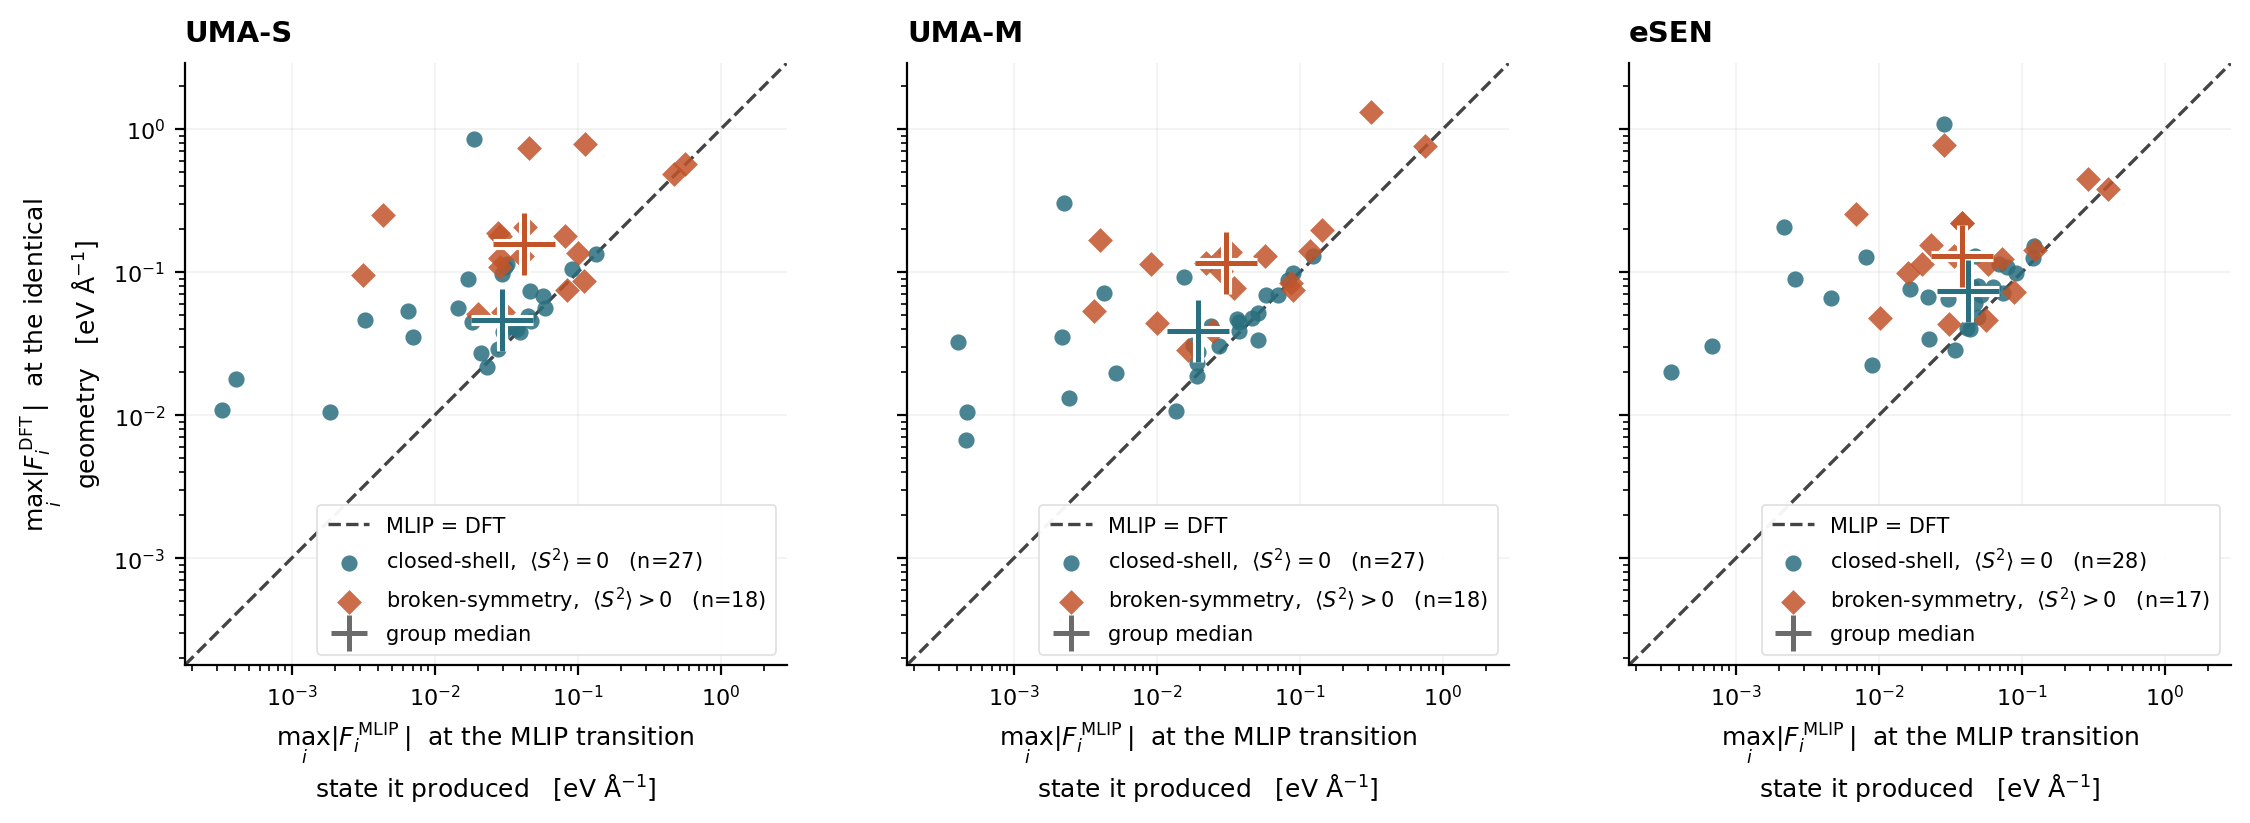
\includegraphics[width=\linewidth]{Pictures/Fig1.png}
  \caption{Residual force according to the model against the residual force
  from the DFT re-evaluation at the identical, unrelaxed geometry --- the
  transition state each model produced (45~reactions $\times$ 3~models, all
  135 structures shown). Both axes give $\max_i |F_i|$ over all $3N$
  Cartesian components. DFT at the OMol25 level on the surface selected by
  the stability analysis (Sec.~\ref{sec:dft}); colours mark the two groups of
  Section~\ref{sec:classification}, $\langle S^2\rangle = 0$ for 82 structures
  and $\geq 0.0579$ for 53. Crosses are group medians, model/DFT, closed-shell
  then broken-symmetry: UMA-S 0.030/0.046, 0.042/0.157; UMA-M 0.019/0.039,
  0.030/0.115; eSEN 0.042/0.074, 0.038/0.129.}
  \label{fig:silent}
\end{figure}


\begin{figure}[t]
  \centering
  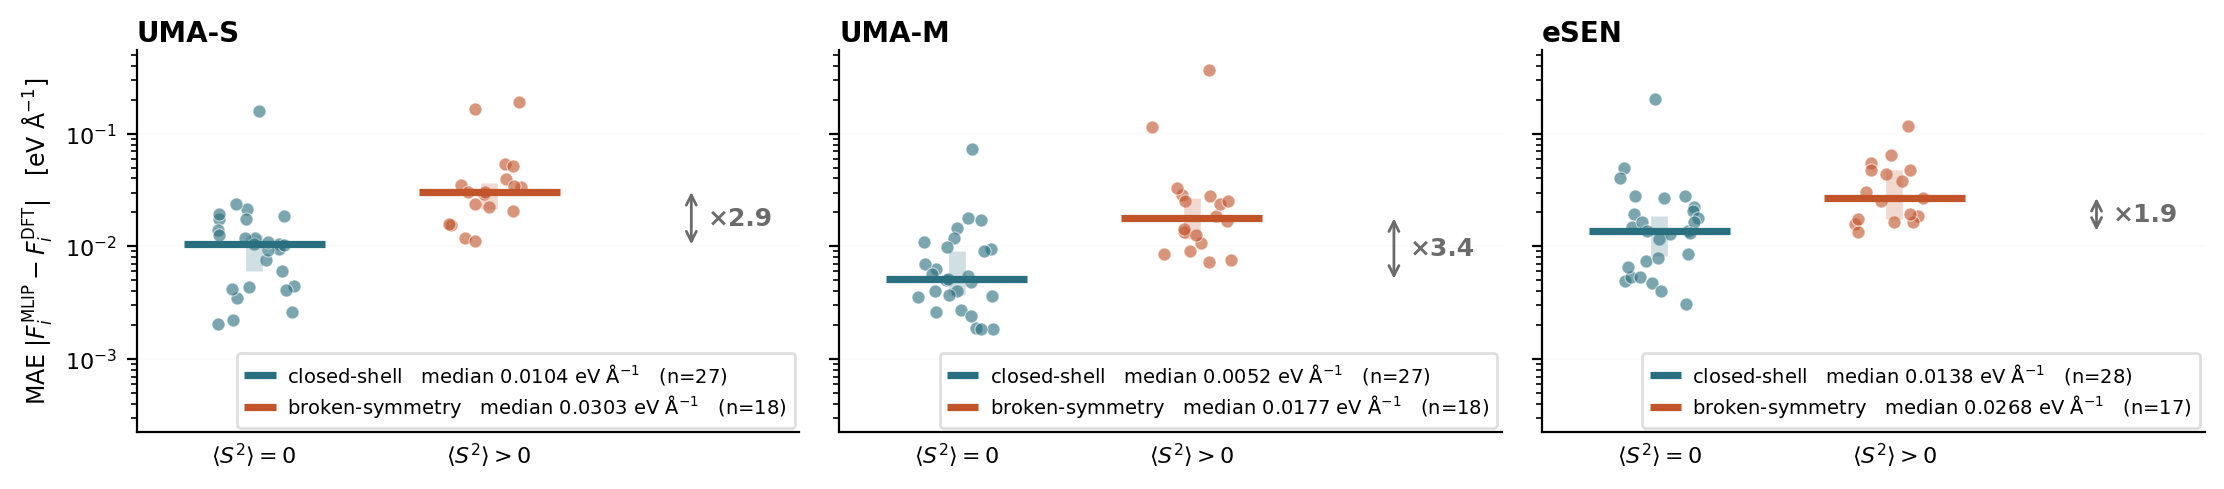
\includegraphics[width=\linewidth]{Pictures/fig2_force_mae.png}
  \caption{Force error at the transition state each model produced: mean
  absolute difference between the model force and the DFT force,
  $\langle |F_i^\mathrm{MLIP} - F_i^\mathrm{DFT}| \rangle_i$ over all $3N$
  Cartesian components, both read at the identical, unrelaxed geometry. DFT
  at the OMol25 level on the surface selected by the stability analysis
  (Sec.~\ref{sec:dft}); groups by $\langle S^2\rangle$ of that single point
  as in Fig.~\ref{fig:silent}. Dots are individual structures, jittered
  horizontally only; bars are group medians, shaded bands their 95\,\%
  bootstrap intervals (10\,000 resamples); the arrow gives the ratio of the
  two medians.}
  \label{fig:ferr}
\end{figure}

\subsection{The force error is larger at broken-symmetry transition states, by a factor of two to three}

Figure~\ref{fig:ferr} shows more directly why the models struggle to find
the broken-symmetry transition states accurately: the quality of the force
prediction deteriorates there. It measures the distance between the force the
model predicts and the force DFT gives at the same geometry --- the two
vectors are subtracted component by component and the absolute differences
averaged over all $3N$ components. Figure~\ref{fig:silent} compared two maxima
that may sit on different atoms; this compares the fields themselves, so it
is zero only if they coincide.

The error is larger at the broken-symmetry structures in every model: medians
of 0.0104 against 0.0303~eV\,\AA$^{-1}$ for UMA-S, 0.0052 against 0.0177 for
UMA-M and 0.0138 against 0.0268 for eSEN --- factors of 2.9, 3.4 and 1.9.
Pooled over the three models the median rises from 0.0095 to 0.0250, and the
largest single component from 0.0353 to 0.1034~eV\,\AA$^{-1}$.

In absolute terms the error stays small, and the two distributions overlap:
4 of the 53 broken-symmetry structures lie below the closed-shell median, 8 of
the 82 closed-shell structures above the broken-symmetry one, and the interval
between the smallest broken-symmetry and the largest closed-shell value holds
100 of the 135 structures. Small as it is, Fig.~\ref{fig:barrier} shows what
it does to the barrier.

Two things follow. The failure in Fig.~\ref{fig:silent} is not a convergence
artefact: the learned force field differs from the ground-state field at the
identical geometry, before any optimisation enters. And the error does not
scale with the breaking depth, which spans 0.6 to 3986~meV within the
broken-symmetry group (Spearman $\rho = -0.05$ over the 53 structures): what
matters is that a second solution exists, not how deep it lies.

\begin{figure}[t]
  \centering
  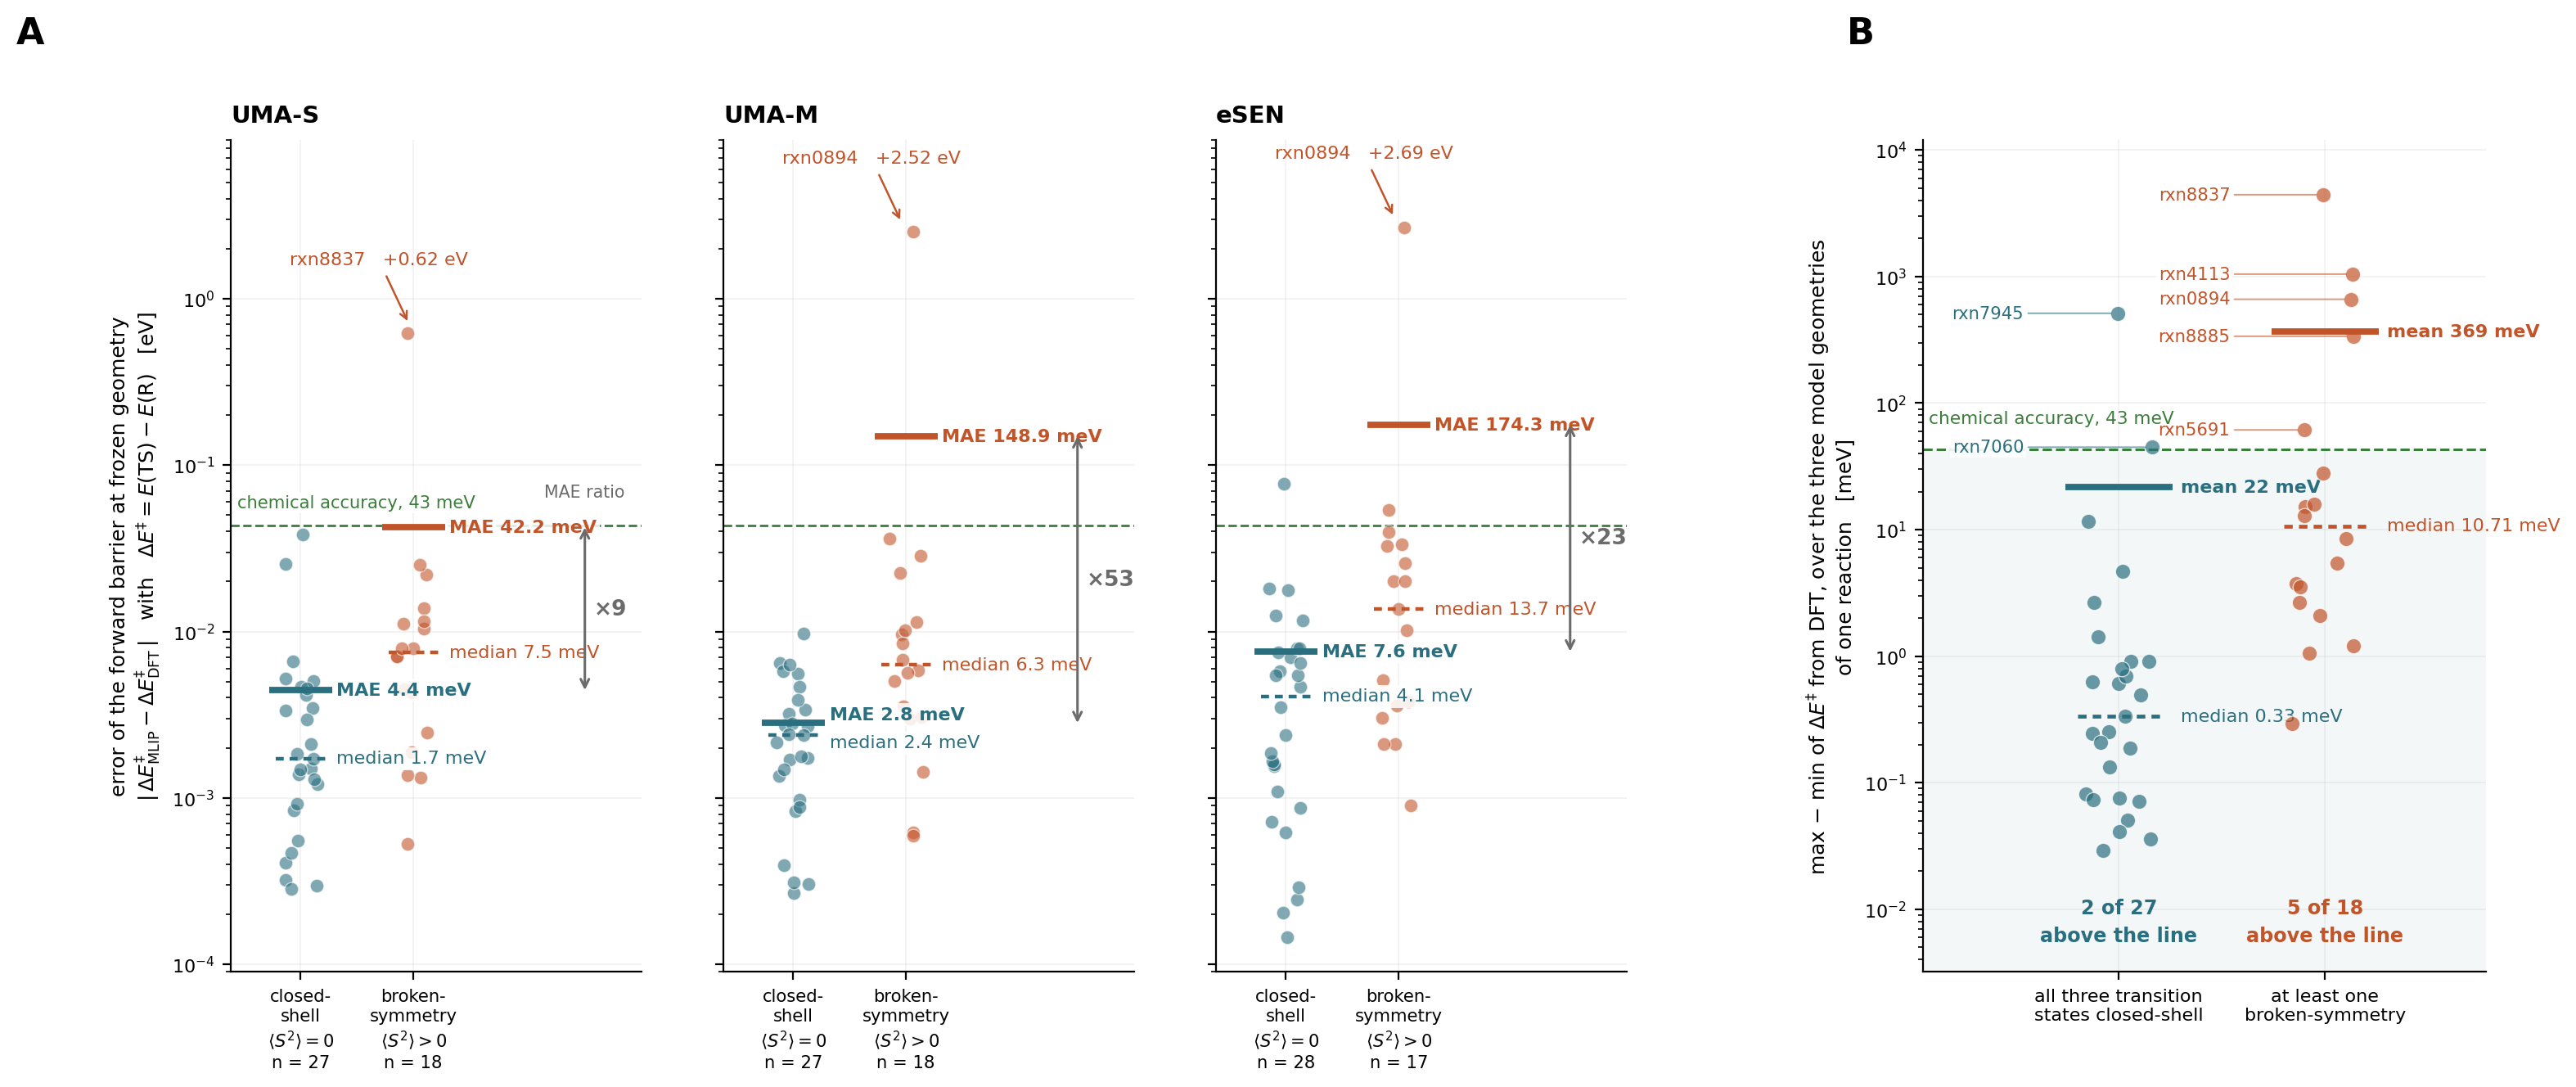
\includegraphics[width=\linewidth]{Pictures/fig3.png}
  \caption{Energy error (A) and geometry error (B) of the model barriers.
  (A)~One dot is one reaction and one model: the structures of that model,
  evaluated with the model and with DFT,
  $|\Delta E^\ddagger_\mathrm{model} - \Delta E^\ddagger_\mathrm{DFT}|$.
  Solid bars are means, dashed bars medians; the named reaction sets the
  mean of each broken-symmetry group almost alone.
  (B)~One dot is one reaction: the structures of all three models,
  evaluated with DFT only, $\max - \min$ of the three barriers. A reaction
  counts as broken-symmetry if at least one of its three transition states
  has $\langle S^2\rangle > 0$.
  The green line marks 1~kcal/mol (43~meV) for orientation only. DFT at the
  OMol25 level on the surface selected by the stability analysis
  (Sec.~\ref{sec:dft}).}
  \label{fig:barrier}
\end{figure}


\subsection{The energy error is small and the geometry error is not}

A model barrier can be wrong for two reasons. The model can assign the wrong
energy to a given structure, or it can place the transition state at the
wrong structure. Figure~\ref{fig:barrier} separates the two.

Panel~A answers the question whether the model assigns the right energy by
keeping the geometries fixed. It takes the reactant and transition state
one model found for a given reaction and evaluates both in two ways, with
the model itself and with a DFT single point. The difference between the
two barriers is the energy error.

Panel~B answers the question how far the barriers differ solely because of
the geometries the models found, this time by keeping the energy evaluation
fixed. For each reaction we take the three sets of reactant and transition
state the three models gave and evaluate the barrier of each with DFT. Any
disagreement between the three barriers now comes from the structures
alone.

\begin{table}[t]
  \centering
  \small
  \begin{tabular}{@{}lll@{}}
    \toprule
                          & Panel A                        & Panel B \\
    \midrule
    Structures (R, TS)    & from one model                 & from the three models \\
    Energy evaluated with & model \emph{and} DFT           & DFT only \\
    Barriers per reaction & 2 per model (6 in total)       & 3 \\
    Fixed                 & the structures                 & the energy function \\
    Varied                & the energy function            & the structures \\
    Plotted               & $|\Delta E^\ddagger_\mathrm{model} - \Delta E^\ddagger_\mathrm{DFT}|$
                          & $\max - \min$ of the three DFT barriers \\
    Measures              & energy error                   & geometry error \\
    \bottomrule
  \end{tabular}
  \caption{How the two panels of Fig.~\ref{fig:barrier} separate the two
  sources of barrier error. R = reactant, TS = transition state.}
  \label{tab:panels}
\end{table}

Panel~A shows that the energy is not the problem. The median error is 1.7,
2.4 and 4.1~meV on the closed-shell and 7.5, 6.3 and 13.7~meV on the
broken-symmetry structures, for UMA-S, UMA-M and eSEN, all well inside
chemical accuracy; 49 of the 53 broken-symmetry structures lie below 43~meV.
The mean absolute errors are 9, 53 and 23 times larger on the broken-symmetry
side, but one reaction per model sets them almost alone: rxn8837 misses by
$+0.62$~eV for UMA-S, rxn0894 by $+2.52$~eV for UMA-M and by $+2.69$~eV for
eSEN. Apart from these three cases the energies are right, also where the
forces are not.

Panel~B shows that the different geometries do cause substantially
diverging barriers. The median spread is 0.33~meV at the closed-shell
reactions and 10.71~meV at the broken-symmetry ones, a factor of 32; the
means are 22 and 369~meV. Five of the 18 broken-symmetry reactions exceed
chemical accuracy, from 61~meV up to 4434~meV, against two of the 27
closed-shell ones, rxn7945 and rxn7060. The drift is concentrated in the
broken-symmetry group but not confined to it. The two reactions with the
largest energy error in Panel~A, rxn8837 and rxn0894, are also among the
three largest spreads in Panel~B.

Together, the two panels say where the barrier error comes from. The energy
error is a few meV; the geometry error reaches electronvolts. The barrier
error is a geometry error. This has a practical consequence. A common
remedy for an inaccurate model energy is a DFT single point at the model
transition state. Here it corrects the energy, which was already right, and
keeps the geometry, which is wrong. The affected transition states have to
be re-optimised, and Fig.~\ref{fig:silent} has shown that the model's own
residual force does not tell which ones they are.

\subsection{The training labels have no stationary point where the models fail}

Table~\ref{tab:ladder} reports the residual force at the Transition1x
transition states, step by step (Sec.~\ref{sec:labels}).

At their own level the geometries are saddle points: median residual force
$0.0147$~eV\,\AA$^{-1}$ for the closed-shell and $0.0138$ for the
broken-symmetry reactions, 44 of 45 below $0.05$. At the OMol25 level on the
restricted surface no geometry is stationary; the median is $0.59$ and the
smallest value $0.196$. This is the level change, and it is the same for
both groups, $0.609$ for the closed-shell and $0.589$ for the broken-symmetry
reactions. On the surface OMol25 labels with, the closed-shell group keeps
its value, since its ground state is the restricted solution. For the 18
broken-symmetry reactions the ground state is the broken-symmetry solution, and
there the residual force is $1.636$, a factor of $2.80$ above the restricted
surface.

Re-optimising on the restricted surface removes the level change: the
restricted residual force drops to $0.039$ and $0.042$ in the two groups.
The ground-state residual force of the broken-symmetry reactions does not.
It is $1.87$ at the re-optimised saddles, a factor of $32$ above the
restricted surface at the same point.

The training geometries of the broken-symmetry reactions therefore lie on a
slope of the surface they are labelled with, before and after the level is
corrected. The models were trained on these points. For the broken-symmetry
reactions the training set contains no transition state at which the
labelled force is zero, only structures near the restricted saddle with
forces of $1.6$ to $1.9$~eV\,\AA$^{-1}$ on them. These are the reactions at
which Figs.~\ref{fig:silent} to \ref{fig:barrier} found the model
transition states off the saddle, with a barrier that depends on where the
model put them, and with a model residual force that reported convergence.

\begin{table}[t]
  \centering
  \small
  \setlength{\tabcolsep}{5pt}
  \begin{tabular}{@{}lccc@{}}
    \toprule
    & \multicolumn{3}{c}{median residual force [eV\,\AA$^{-1}$], evaluated with} \\
    \cmidrule(l){2-4}
    & Transition1x level & OMol25 level & OMol25 level \\
    & $\omega$B97X-D3/6-31G(d) & $\omega$B97M-V/def2-TZVPD & $\omega$B97M-V/def2-TZVPD \\
    & restricted & restricted & ground-state surface$^{a}$ \\
    & (as relaxed) & (level changed) & (as labelled by OMol25) \\
    \midrule
    \multicolumn{4}{@{}l}{\emph{Transition1x transition states, relaxed at the Transition1x level} (45)} \\
    \quad closed-shell (27)     & $0.0147$ & $0.609$ & $0.609$ \\
    \quad broken-symmetry (18)  & $0.0138$ & $0.589$ & $1.636$ \\
    \addlinespace
    \multicolumn{4}{@{}l}{\emph{Re-optimised at the OMol25 level, restricted surface} (33)} \\
    \quad closed-shell (18)     & -- & $0.039$ & $0.039$ \\
    \quad broken-symmetry (15)  & -- & $0.042$ & $1.87$ \\
    \bottomrule
  \end{tabular}
  \caption{Residual force at the transition-state geometries, read from left
  to right: at the level the geometries were relaxed at, after changing the
  level, and on the surface OMol25 labels with. The second block
  re-optimises the saddles at the OMol25 level on the restricted surface,
  which removes the level change; numbers in parentheses are reaction
  counts. $^{a}$Surface selected by the stability analysis
  (Sec.~\ref{sec:dft}): restricted for the closed-shell group, so the last
  two columns coincide there, and unrestricted for the broken-symmetry
  group.}
  \label{tab:ladder}
\end{table}

Transition1x is not the only reactive data in OMol25, and one might
object that the models learned the broken-symmetry saddles elsewhere.
They could not. No geometry in OMol25 was relaxed at the level the
labels use; every structure was labelled where it stood, whether taken
from an existing dataset or generated with a cheaper
method~\cite{omol25}. The organic reaction paths are Transition1x, the
Grambow reactions and RGD1, whose transition states were all optimised
restricted and whose intermediate geometries are interpolated between
reactant, transition state and product rather than relaxed, so the
only saddle on each path is the restricted one. The reaction paths
OMol25 generated itself come from artificial-force searches and
semi-empirical optimisation, relaxed on no DFT surface at all. A
saddle of the ground-state surface at the OMol25 level therefore does
not exist in the training data.
